\documentclass[11pt,a4paper]{article}
\usepackage[margin=2.4cm]{geometry}
\usepackage[T1]{fontenc}
\usepackage{lmodern}
\usepackage{graphicx}
\usepackage{booktabs}
\usepackage{tabularx}
\usepackage{caption}
\usepackage{xcolor}
\usepackage[hidelinks]{hyperref}
\usepackage{enumitem}
\usepackage{float}
\usepackage{fancyhdr}
\pagestyle{fancy}\fancyhf{}\cfoot{Page \thepage}\renewcommand{\headrulewidth}{0pt}
\definecolor{navy}{HTML}{0B2A4A}
\setlength{\parskip}{4pt}
\begin{document}
\begin{titlepage}\centering\vspace*{2cm}
{\color{navy}\large Applied AI Research Workshop - Module 1 Methodology and Implementation Report\par}\vspace{0.8cm}
{\color{navy}\LARGE\bfseries Vision Transformer-Based Visual Analysis of Hybrid-Slotted DGS Compact Patch Antennas\par}\vspace{0.5cm}
{\large Module 1 of the Applied Vision Transformer Framework for 5G and Emerging 6G Networks - Proof-of-Concept Prototype\par}\vspace{1cm}
{\bfseries Module 1: Image-Based Vision Transformer for Antenna Performance Classification and Explainable Visual Analysis\par}\vspace{2cm}
\begin{tabular}{ll}
\textbf{Student name} & [to be completed by student] \\
\textbf{Student ID} & [to be completed by student] \\
\textbf{Programme / Module} & [to be completed by student] \\
\textbf{Institution} & [to be completed by student] \\
\textbf{Submission date} & [to be completed by student] \\
\textbf{Report generated} & 26 October 2026 \\
\textbf{Code repository} & \url{https://github.com/rathiabeth/module1-vit-antenna-image-classification} \\
\end{tabular}\vfill
{\small Bracketed fields are deliberate placeholders for personal details that were not provided. All results are from executed experiments on public simulation data. Ansys HFSS was not available and was not run.\par}
\end{titlepage}
\tableofcontents\newpage
\section*{Abstract}\addcontentsline{toc}{section}{Abstract}
This report documents the implementation and evaluation of Module 1 of a two-module applied-AI framework for hybrid-slotted defected ground structure (DGS) compact patch antennas: an image-based Vision Transformer (ViT) that classifies antenna performance from standardised images and explains which image regions drive its predictions. No licensed public dataset of Ansys HFSS images of hybrid-slotted DGS antennas exists, and HFSS was not available, so the module was built and executed as a proof of concept on two verified public simulation datasets: 2,051 openEMS-simulated rectangular patch antennas (MIT licence) and 3,000 RadPat-50K radiation-pattern plots (CC BY 4.0). Every patch design was rendered as a text-free, standardised two-panel geometry image and labelled from its simulated S11 response using rules frozen before training. A ViT-S/16 pretrained on ImageNet-21k was partially fine-tuned on a CPU and compared with a majority-class baseline, a compact CNN and a frozen-backbone linear probe on a locked design-level split. On the three-class impedance-matching task the pre-registered fine-tuned ViT reached a test macro-F1 of 0.582 $\pm$ 0.008 (three seeds), against 0.643 $\pm$ 0.022 for the CNN, 0.709 for the linear probe and 0.269 for the majority baseline. Training curves showed underfitting, and the augmentation ablation identified the cause: small rotations and shifts blurred the one-to-two-pixel feed offset that determines matching. Without augmentation the same ViT reached 0.725 (exploratory, one seed). Attention rollout placed 1.41 times more attribution on the feed region than its area share in the median design, but also revealed background attention sinks. Robustness tests showed sensitivity to blur and colour rendering. The results establish a reproducible, honest image pipeline that is ready to be applied to the HFSS dataset; they do not validate hybrid-slotted DGS performance.

\textbf{Keywords:} Vision Transformer; patch antenna; defected ground structure; explainability; attention rollout; 5G/6G.

\section*{1. Introduction and Recap of the Research Problem}\addcontentsline{toc}{section}{1. Introduction and Recap of the Research Problem}
Compact printed patch antennas are central to 5G and emerging 6G devices. Slots and defected ground structures reshape surface-current paths and can tune resonance, impedance matching and bandwidth [4], but small geometric changes can produce large electromagnetic differences. Full-wave solvers such as Ansys HFSS give physically grounded answers, yet large design sweeps are slow. The Module 1 research report proposed a complementary tool: a pretrained Vision Transformer [1] that reads standardised antenna geometry and electromagnetic field images, predicts a documented performance class, and shows which regions of the image influence each prediction. The tool is a rapid screening aid, not a replacement for full-wave simulation.

The research objective of this module is unchanged from that report: \textbf{to investigate whether standardised antenna geometry and electromagnetic images can support antenna-performance classification and explainable visual analysis.} Module 1 is the image branch of the overall framework. The numerical-text surrogate, the multimodal fusion stage and the NSGA-II optimisation form Module 2, which is documented in a separate report and repository (\url{https://github.com/rathiabeth/module2-numerical-surrogate-antenna-design}). The only artefact Module 1 passes to Module 2 is the 384-dimensional image embedding of each design.

\begin{table}[H]\centering\small
\caption*{Table 1. Implementation status of Module 1.}
\begin{tabularx}{\linewidth}{XXX}
\toprule
\textbf{Component} & \textbf{Status} & \textbf{Evidence in repository} \\
\midrule
Dataset discovery and licence verification & Completed & \href{https://github.com/rathiabeth/module1-vit-antenna-image-classification/blob/main/docs/DATASET_SURVEY.md}{docs/DATASET\_SURVEY.md} \\
Preprocessing, standardised images, labels, locked splits & Completed and executed & \href{https://github.com/rathiabeth/module1-vit-antenna-image-classification/blob/main/src/preprocessing.py}{src/preprocessing.py}, \href{https://github.com/rathiabeth/module1-vit-antenna-image-classification/blob/main/src/dataset.py}{src/dataset.py}, \href{https://github.com/rathiabeth/module1-vit-antenna-image-classification/tree/main/data}{data} \\
ViT-S/16 partial fine-tuning and frozen linear probe & Completed and executed & \href{https://github.com/rathiabeth/module1-vit-antenna-image-classification/blob/main/src/train_vit.py}{src/train\_vit.py}, \href{https://github.com/rathiabeth/module1-vit-antenna-image-classification/tree/main/results/metrics}{results/metrics} \\
Majority and compact CNN baselines & Completed and executed & \href{https://github.com/rathiabeth/module1-vit-antenna-image-classification/blob/main/src/train_baseline.py}{src/train\_baseline.py} \\
Statistical comparison (McNemar, bootstrap CI) & Completed and executed & \href{https://github.com/rathiabeth/module1-vit-antenna-image-classification/blob/main/src/evaluate.py}{src/evaluate.py} \\
Attention rollout, robustness and OOD tests & Completed and executed & \href{https://github.com/rathiabeth/module1-vit-antenna-image-classification/blob/main/src/explainability.py}{src/explainability.py} \\
Automated tests & Completed and executed & \href{https://github.com/rathiabeth/module1-vit-antenna-image-classification/tree/main/tests}{tests}, \href{https://github.com/rathiabeth/module1-vit-antenna-image-classification/blob/main/results/test_report.txt}{results/test\_report.txt} \\
Embedding export for Module 2 fusion & Completed and executed & \href{https://github.com/rathiabeth/module1-vit-antenna-image-classification/tree/main/results/features}{results/features} \\
HFSS hybrid-slotted DGS images (geometry, current, E-field) & Proposed (HFSS unavailable) & Section 11 \\
Block diagram (Figure 1) & Illustrative & \href{https://github.com/rathiabeth/module1-vit-antenna-image-classification/blob/main/results/figures/module1_architecture.png}{results/figures/module1\_architecture.png} \\
\bottomrule
\end{tabularx}
\end{table}
\begin{figure}[H]\centering
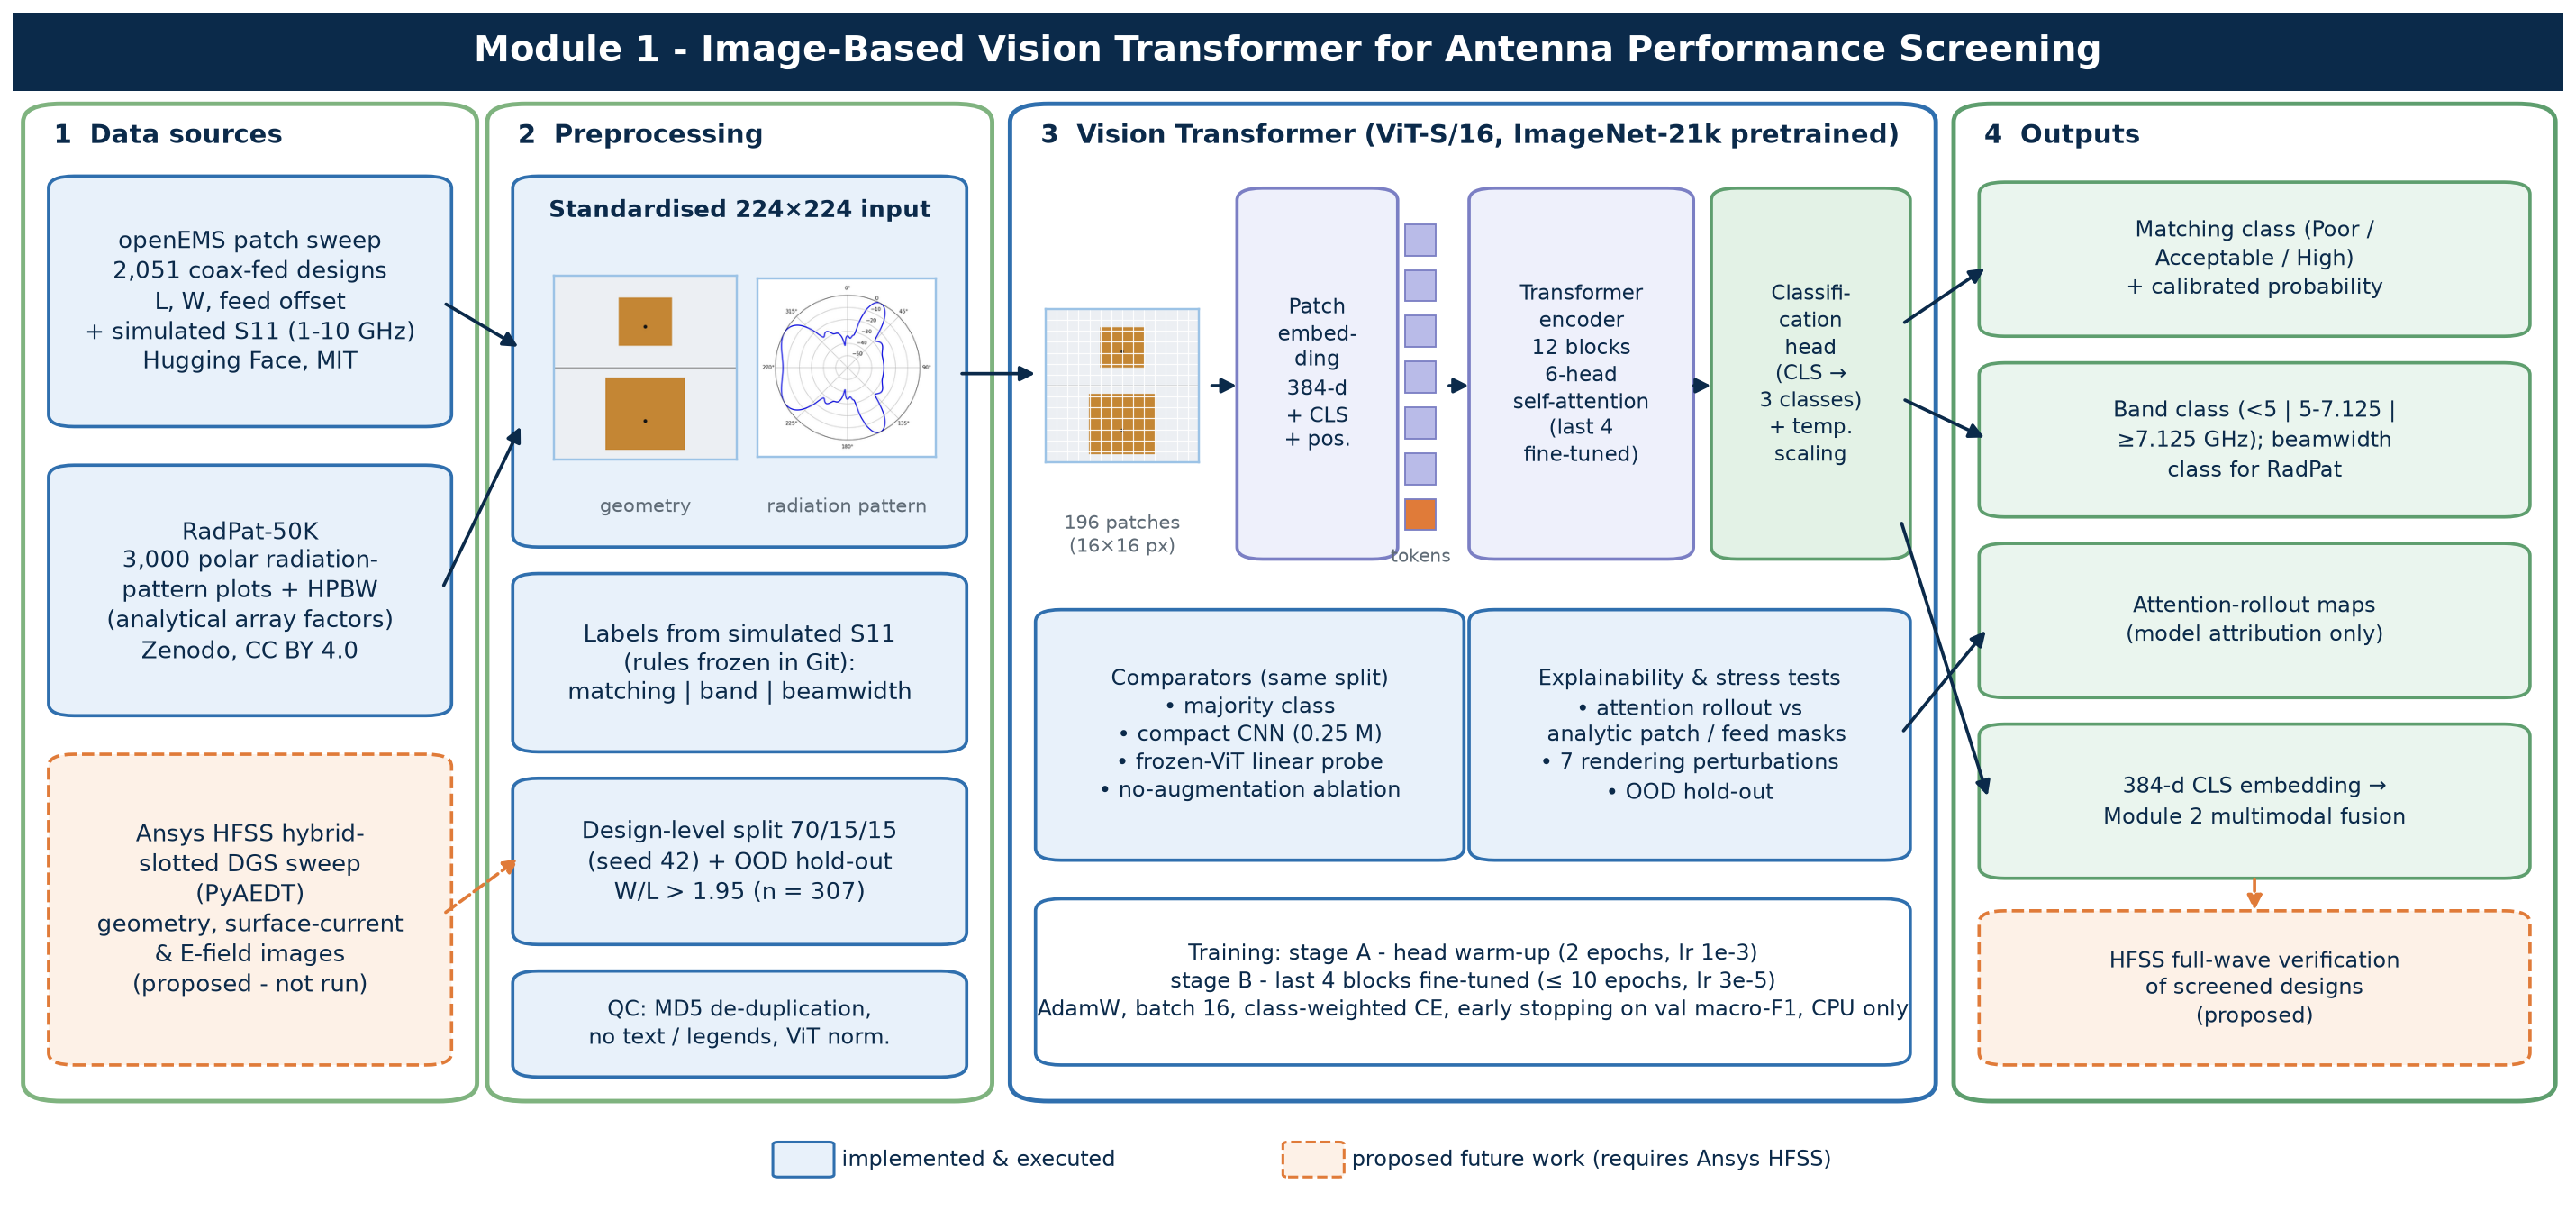
\includegraphics[width=1.00\linewidth]{../results/figures/module1_architecture.png}
\caption*{Figure 1. Module 1 block diagram. Solid boxes were implemented and executed; dashed orange boxes are proposed work that requires Ansys HFSS. The thumbnails are real model inputs.}
\end{figure}
\section*{2. Research Design and Hypotheses}\addcontentsline{toc}{section}{2. Research Design and Hypotheses}
The study follows an applied, experimental machine-learning design. The independent variables are the model family (majority class, compact CNN, frozen ViT with a linear probe, partially fine-tuned ViT), the image modality (geometry drawing or radiation-pattern plot) and the evaluation distribution (in-distribution test split or out-of-distribution hold-out). The dependent variables are classification metrics on simulated performance classes. The research questions, hypotheses, label rules, split and seed were committed to Git before any fine-tuned result existed (docs/HYPOTHESES.md). One frozen linear-probe test score had been printed beforehand; this is disclosed in that file.

\begin{table}[H]\centering\small
\caption*{Table 2. Research questions and their operationalisation.}
\begin{tabularx}{\linewidth}{XXX}
\toprule
\textbf{RQ} & \textbf{Question} & \textbf{Operationalisation} \\
\midrule
RQ1 & Can standardised antenna images predict documented performance classes? & Geometry image $\rightarrow$ matching class and band class \\
RQ2 & Does a pretrained ViT outperform a compact CNN? & Same split, three seeds each, exact McNemar test, bootstrap CI \\
RQ3 & Which available image modality gives the strongest signal? & Geometry vs radiation-pattern images (descriptive only: different datasets) \\
RQ4 & Do attention maps highlight physically relevant regions? & Rollout mass inside analytic patch and feed masks vs their area share \\
RQ5 & How robust are the predictions? & OOD hold-out (W/L > 1.95) and seven rendering perturbations \\
\bottomrule
\end{tabularx}
\end{table}
The directional hypotheses tested on the locked test split were:

\begin{itemize}[leftmargin=*,itemsep=1pt]
\item \textbf{H1}: ViT > majority baseline (both patch tasks).
\item \textbf{H2}: ViT $\geq$ compact CNN (3-seed mean, matching class).
\item \textbf{H3}: Partial fine-tune > frozen linear probe.
\item \textbf{H4}: Attention enriched on patch and feed (median > 1).
\item \textbf{H5}: Lower macro-F1 on OOD (W/L > 1.95).
\end{itemize}
A sixth pre-registered hypothesis (H6: fusing image embeddings with numerical features improves on the image-only classifier) concerns the fusion stage and is reported in the Module 2 report.

\section*{3. Dataset Description and Source Verification}\addcontentsline{toc}{section}{3. Dataset Description and Source Verification}
Repositories were searched in the order set by the brief (Hugging Face, Kaggle, Mendeley Data, IEEE DataPort, GitHub), with Zenodo added. Eleven candidates were recorded with title, repository, version, authors, licence, size, features and limitations (docs/DATASET\_SURVEY.md). Candidates were judged on relevance to the research question. Self-declared AI-generated datasets, text-only corpora, non-commercial licences and sets too small for a 70/15/15 split were rejected. No public, licensed dataset of HFSS images of hybrid-slotted DGS antennas with linked performance labels was found. Following the brief's dataset rule, tabular data without images (such as the Mendeley Antenna Parameters Dataset) were assigned to Module 2 and are not presented here as images.

\begin{table}[H]\centering\small
\caption*{Table 3. Datasets used by Module 1 (verified 25 October 2026).}
\begin{tabularx}{\linewidth}{XXXXX}
\toprule
\textbf{Dataset} & \textbf{Source / version} & \textbf{Licence} & \textbf{Content} & \textbf{Role in Module 1} \\
\midrule
Rectangular Patch Antenna Frequency Response [2] & Hugging Face becklabash/rectangular-patch-antenna-freq-response, rev. 4be72a2 & MIT & 2,051 coax-fed patches; L, W, feed offset; 1,000-point S11 (1--10 GHz), openEMS FDTD; $\varepsilon$r 3.68, h 1.61 mm & Geometry images, matching and band labels \\
RadPat-50K [3] & Zenodo 10.5281/zenodo.17067881, v1.1 & CC BY 4.0 & Uniform-linear-array polar plots with metadata; 10K polar subset, 3,000 sampled & Radiation-pattern image modality, beamwidth labels \\
\bottomrule
\end{tabularx}
\end{table}
\textbf{Nature of the evidence.} The patch data are full-wave FDTD simulations produced with openEMS [11]. RadPat consists of analytically computed array factors with injected noise, so it is synthetic. None of the data is measured, and no HFSS output is claimed.

\textbf{Discrepancies recorded during verification.} The patch dataset README gives L $\in$ [7.5, 52.5] mm and p $\in$ [-6, 0) mm; the observed values are L $\in$ [7.5, 47.5] mm and p $\in$ [-15.83, 0] mm, including 100 centre-fed designs. The README states $\varepsilon$r = 3.68 while the repository diagram shows 3.38. 1170 S11 curves exceed 0 dB by at most 0.2 dB, a passive-port numerical artefact. In RadPat, 5,015 of 10,000 rows carry a -120 dBi directivity sentinel, so directivity was not used as a label.

\section*{4. Data Preprocessing and Preparation}\addcontentsline{toc}{section}{4. Data Preprocessing and Preparation}
\subsection*{4.1 Targets and label rules}\addcontentsline{toc}{subsection}{4.1 Targets and label rules}
Each simulated S11 curve was reduced to the global minimum S11 (S11min), the \textbf{first matched resonance} f\_res (the lowest-frequency local minimum below -10 dB), S11 at f\_res and the contiguous -10 dB bandwidth. The first matched resonance was used because the deepest dip is often a higher-order mode; for example, a 22.5 mm patch showed its deepest dip at 9.6 GHz. Labels were defined by explicit rules frozen before training:

\begin{itemize}[leftmargin=*,itemsep=1pt]
\item \textbf{Matching class} (main task): Poor if S11min > -10 dB; Acceptable if -20 dB < S11min $\leq$ -10 dB; High if S11min $\leq$ -20 dB. -10 dB (VSWR $\approx$ 1.9) is the conventional impedance-bandwidth criterion. The -20 dB boundary is a \textbf{project assumption} that requires engineering confirmation before the classes are treated as physically validated.
\item \textbf{Band class} (secondary task): f\_res < 5 GHz (covers NR n77/n78/n79), 5--7.125 GHz (upper FR1), $\geq$ 7.125 GHz (FR3, a 6G candidate range), with edges taken from 3GPP TS 38.101-1 [5].
\item \textbf{Beamwidth class} (RadPat): half-power beamwidth terciles computed on the training split only ($\leq$ 6.48$^\circ$, $\leq$ 17.82$^\circ$, above).
\end{itemize}
\subsection*{4.2 Standardised geometry images}\addcontentsline{toc}{subsection}{4.2 Standardised geometry images}
Each design was rendered as a 224 $\times$ 224 RGB image with two panels. The top panel is an absolute-scale top view at a fixed 1.962 px/mm, so physical size, which governs resonance, is visible. The bottom panel shows the same patch scaled to fill the frame, so the relative feed position, which governs matching, can be resolved at the 16-pixel patch size of the ViT. Background, copper and feed colours are fixed, and there is no text, legend, axis or filename, which removes label leakage through annotations. Rendering at 4$\times$ and downsampling with a Lanczos filter preserves sub-pixel feed position through anti-aliasing. These images are drawings of the simulated geometry, not field exports. RadPat polar plots were verified, converted to RGB and resized to 224 $\times$ 224.

\begin{figure}[H]\centering
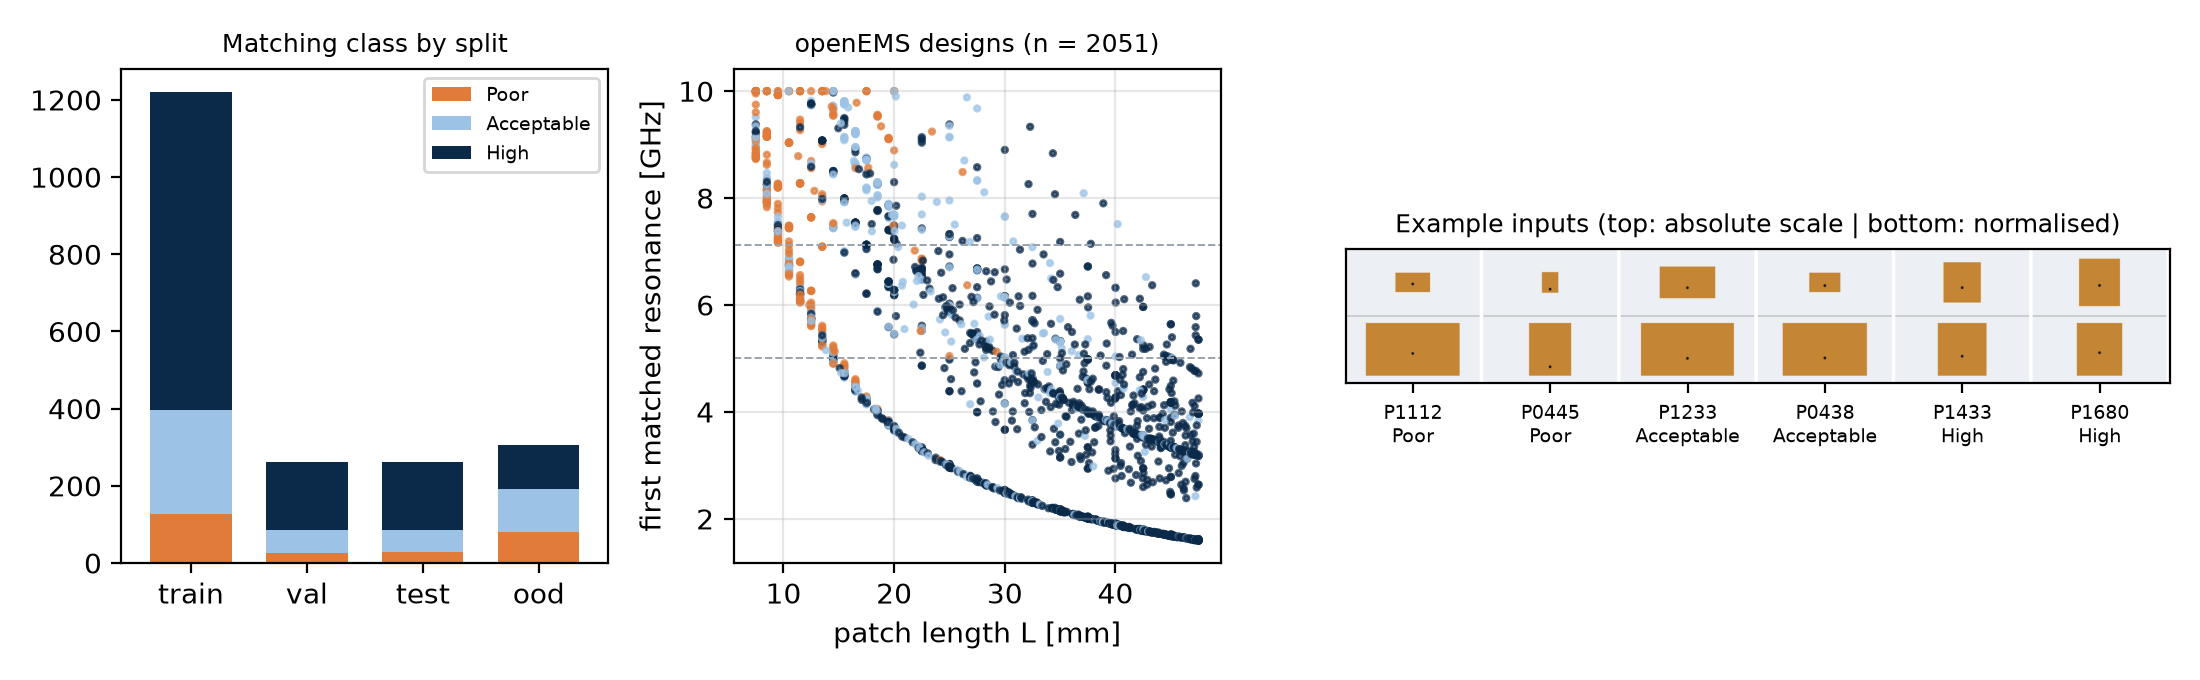
\includegraphics[width=1.00\linewidth]{../results/figures/dataset_overview.png}
\caption*{Figure 2. Class distribution by split, design space (patch length vs first matched resonance; dashed lines are band edges) and example standardised inputs.}
\end{figure}
\begin{figure}[H]\centering
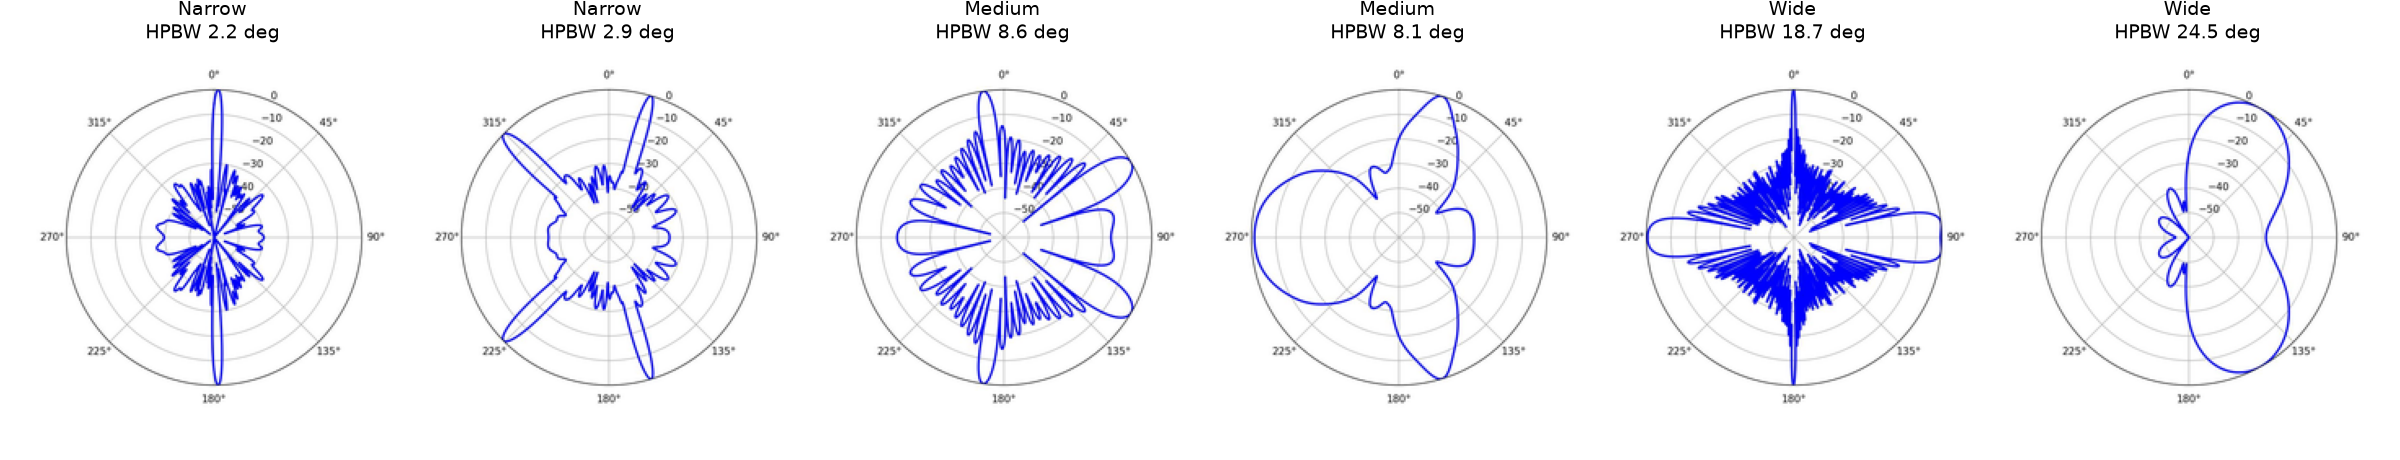
\includegraphics[width=0.89\linewidth]{../results/figures/radpat_samples.png}
\caption*{Figure 3. Example RadPat-50K polar plots from the training split with their beamwidth class.}
\end{figure}
\subsection*{4.3 Cleaning, duplicates and leakage control}\addcontentsline{toc}{subsection}{4.3 Cleaning, duplicates and leakage control}
\begin{itemize}[leftmargin=*,itemsep=1pt]
\item Patch: 2,051 rows, 0 non-finite curves, 0 duplicate parameter triples and 0 identical rendered images (MD5). Identical images would have been forced into one split.
\item Perceptual hashing produced 21,561 colliding pairs because the images are simple rectangles, so it was judged unsuitable for near-duplicate grouping. Splitting relies on exact design identity; near-neighbour interpolation is discussed as a limitation.
\item RadPat: all 3,000 sampled images passed PIL verification and a blank-image check; 0 exact duplicates.
\item Split: every design with W/L > 1.95 (n = 307) was removed first as an out-of-distribution hold-out. The rest was split by design, stratified on matching class, 70/15/15 with seed 42 (train 1,220, validation 262, test 262). Each design has exactly one image, so no design can appear in two splits. Manifests are in data/splits.
\item Normalisation used the checkpoint's statistics (mean = std = 0.5 for the AugReg ViT). No statistic was computed on the test split.
\item Training-only augmentation: horizontal mirror (justified because the patch is symmetric about its length axis), rotation of $\pm$3$^\circ$ and translation of up to 2\%. Scale augmentation was excluded because it would change the apparent physical size and therefore the label.
\end{itemize}
The data dictionary is in Appendix A and online at \href{https://github.com/rathiabeth/module1-vit-antenna-image-classification/blob/main/data/data_dictionary.csv}{data/data\_dictionary.csv}. Every count and threshold is logged in \href{https://github.com/rathiabeth/module1-vit-antenna-image-classification/blob/main/data/processed/preprocessing_log.json}{data/processed/preprocessing\_log.json}, the split manifests are in \href{https://github.com/rathiabeth/module1-vit-antenna-image-classification/tree/main/data/splits}{data/splits}, and the rules are enforced by 18 automated tests (Section 10).

\section*{5. Proposed Model: Vision Transformer}\addcontentsline{toc}{section}{5. Proposed Model: Vision Transformer}
The primary model is ViT-S/16 (timm checkpoint vit\_small\_patch16\_224.augreg\_in21k\_ft\_in1k; 21.7 M parameters with the three-class head) [1, 6]. A 224 $\times$ 224 image is split into 14 $\times$ 14 = 196 non-overlapping 16 $\times$ 16 patches. These are linearly embedded to 384 dimensions, prepended with a classification (CLS) token, given learned positional embeddings and processed by 12 pre-norm transformer blocks with six-head self-attention. A new linear head (dropout 0.1) maps the CLS token to class logits. Self-attention lets the feed region attend directly to the patch edges, which are not adjacent in the image; the reference report identified this as the property that makes a ViT attractive for antenna layouts. ViT-Small (the size class of DeiT-Small [10]) was chosen over ViT-Base because the dataset is small and specialised and training ran on a CPU.

\textbf{Outputs.} For each image the model returns temperature-scaled class probabilities, the predicted class, its confidence and the 384-dimensional CLS embedding. Predictions are saved to results/predictions and embeddings to results/features; the embeddings of the pre-registered seed-42 model are the input to Module 2's fusion stage.

\textbf{Explainability.} Attention rollout [7] multiplies the head-averaged attention matrices (plus identity) across all 12 blocks and reads the CLS row. For a quantitative check, an analytic patch mask and a 6-pixel feed halo are computed from each design's parameters. Enrichment is the share of rollout mass inside a region divided by that region's area share; a value of 1 means no preference. Attention is treated as model attribution, never as evidence of electromagnetic causation.

\section*{6. Training Strategy and Experimental Setup}\addcontentsline{toc}{section}{6. Training Strategy and Experimental Setup}
\begin{table}[H]\centering\small
\caption*{Table 4. Pre-registered ViT training configuration (configs/default.yaml).}
\begin{tabularx}{\linewidth}{XXX}
\toprule
\textbf{Setting} & \textbf{Value} & \textbf{Note} \\
\midrule
Stage A & 2 epochs, head only, AdamW, lr 1e-3 & Head warm-up \\
Stage B & $\leq$ 10 epochs, last 4 blocks + norm + head & Backbone lr 3e-5, head lr 3e-4, one-cycle cosine \\
Batch size / weight decay & 16 / 0.01 & As recommended in the Module 1 report \\
Loss & Class-weighted cross-entropy & Weights from the training split only \\
Early stopping & Patience 3 on validation macro-F1 & Reduced from 8 because of the CPU budget \\
Calibration & Temperature scaling on validation logits [8] & Applied before test evaluation \\
Seeds & 42, 43, 44 (main task); 42 elsewhere & Split fixed at seed 42 \\
Hardware & Intel i7-10610U CPU, 4 threads, PyTorch [9], no GPU & $\approx$ 25 min for the seed-42 run \\
\bottomrule
\end{tabularx}
\end{table}
Two deviations from the reference plan were made for feasibility and are recorded here: only the upper four transformer blocks were unfrozen, and early-stopping patience was 3 epochs instead of 8. A full hyperparameter grid (learning rate $\times$ weight decay $\times$ dropout) was not run because one fine-tuning run takes about half an hour on the CPU; the recommended defaults were used. Models were selected on validation macro-F1, and the test split was evaluated once per final model.

\textbf{Amendment 1 (disclosed deviation).} The pre-registered seed-42 run underfitted (training accuracy about 0.70 and still rising; best validation macro-F1 0.660, below the linear probe's 0.702). A revised configuration that changes only optimisation settings (backbone learning rate 1e-4, six unfrozen blocks, 15 epochs, patience 5) was added with a validation-only adoption rule: it would replace the pre-registered model only if its validation macro-F1 beat both values. It did not, so the pre-registered model remained final. The augmentation ablation planned in the reference report was also run. Both follow-ups are labelled exploratory.

\section*{7. Baseline Methods and Comparative Models}\addcontentsline{toc}{section}{7. Baseline Methods and Comparative Models}
\begin{itemize}[leftmargin=*,itemsep=1pt]
\item \textbf{Majority class}: always predicts the most frequent training class; the minimum useful result.
\item \textbf{Compact CNN} (trained from scratch, 0.25 M parameters): stride-2 5 $\times$ 5 stem, four 3 $\times$ 3 conv--BN--ReLU--max-pool blocks (32--64--128--128 channels), global average pooling and dropout 0.2; AdamW lr 1e-3, cosine schedule, $\leq$ 25 epochs, patience 5. Same split, augmentation, class weights and calibration as the ViT.
\item \textbf{Frozen ViT linear probe}: CLS features of the pretrained backbone with multinomial logistic regression; C selected on validation macro-F1. It separates what the pretrained representation already knows from what fine-tuning adds.
\item \textbf{Ablations}: the ViT and the CNN retrained without augmentation (seed 42), and the Amendment 1 optimisation profile.
\end{itemize}
\section*{8. Evaluation Metrics and Analysis Plan}\addcontentsline{toc}{section}{8. Evaluation Metrics and Analysis Plan}
Classification is reported with accuracy, macro and weighted precision, recall and F1, balanced accuracy, one-vs-rest macro ROC-AUC, the confusion matrix and expected calibration error (ECE, 10 bins). Macro-F1 is the primary metric because the classes are imbalanced. Results are mean $\pm$ SD over seeds where several seeds were run. The paired ViT--CNN comparison uses an exact McNemar test on test-set correctness [12], and a 95\% percentile bootstrap interval [13] (2,000 resamples of test designs) is given for macro-F1. Robustness is the change in test macro-F1 under each perturbation, together with agreement with the clean-image predictions. The analysis plan was fixed in docs/HYPOTHESES.md before results were produced.

\section*{9. Results and Discussion}\addcontentsline{toc}{section}{9. Results and Discussion}
Every number in this section comes from executed runs stored in results/metrics. No value is estimated or illustrative.

\subsection*{9.1 Main task: geometry image to matching class (RQ1, RQ2)}\addcontentsline{toc}{subsection}{9.1 Main task: geometry image to matching class (RQ1, RQ2)}
\begin{table}[H]\centering\small
\caption*{Table 5. Locked test split (n = 262 designs), matching class. Mean $\pm$ SD over seeds.}
\begin{tabularx}{\linewidth}{XXXXXXX}
\toprule
\textbf{Model} & \textbf{Seeds} & \textbf{Accuracy} & \textbf{Macro-F1} & \textbf{Bal. acc.} & \textbf{ROC-AUC} & \textbf{ECE} \\
\midrule
Majority baseline & 1 & 0.676 & 0.269 & 0.333 & 0.500 & 0.000 \\
Compact CNN & 3 & 0.676 $\pm$ 0.030 & 0.643 $\pm$ 0.022 & 0.669 & 0.799 & 0.063 \\
ViT-S/16 linear probe & 1 & 0.718 & 0.709 & 0.729 & 0.828 & 0.057 \\
ViT-S/16 fine-tuned & 3 & 0.622 $\pm$ 0.014 & 0.582 $\pm$ 0.008 & 0.649 & 0.776 & 0.062 \\
\bottomrule
\end{tabularx}
\end{table}
All learned models clearly beat the majority baseline (macro-F1 0.269), so \textbf{H1} holds for the main task. The fine-tuned ViT reached 0.582 $\pm$ 0.008 against 0.643 $\pm$ 0.022 for the compact CNN (\textbf{H2} -- Not supported: 0.582 $\pm$ 0.008 vs 0.643 $\pm$ 0.022; McNemar p = 0.000912 (seed 42)). The bootstrap 95\% intervals for seed 42 are [0.514, 0.642] for the ViT and [0.589, 0.715] for the CNN. In the exact McNemar test (seed 42) the ViT alone was correct on 5 designs and the CNN alone on 23. Fine-tuning versus the frozen probe: \textbf{H3} -- Not supported: 0.582 vs 0.709; McNemar p = 0.00877.

\begin{table}[H]\centering\small
\caption*{Table 6. Per-class test results, pre-registered fine-tuned ViT (seed 42).}
\begin{tabularx}{\linewidth}{XXXXX}
\toprule
\textbf{Class} & \textbf{Precision} & \textbf{Recall} & \textbf{F1} & \textbf{Support} \\
\midrule
Poor & 0.511 & 0.857 & 0.640 & 28 \\
Acceptable & 0.321 & 0.439 & 0.370 & 57 \\
High & 0.839 & 0.650 & 0.732 & 177 \\
\bottomrule
\end{tabularx}
\end{table}
\begin{figure}[H]\centering
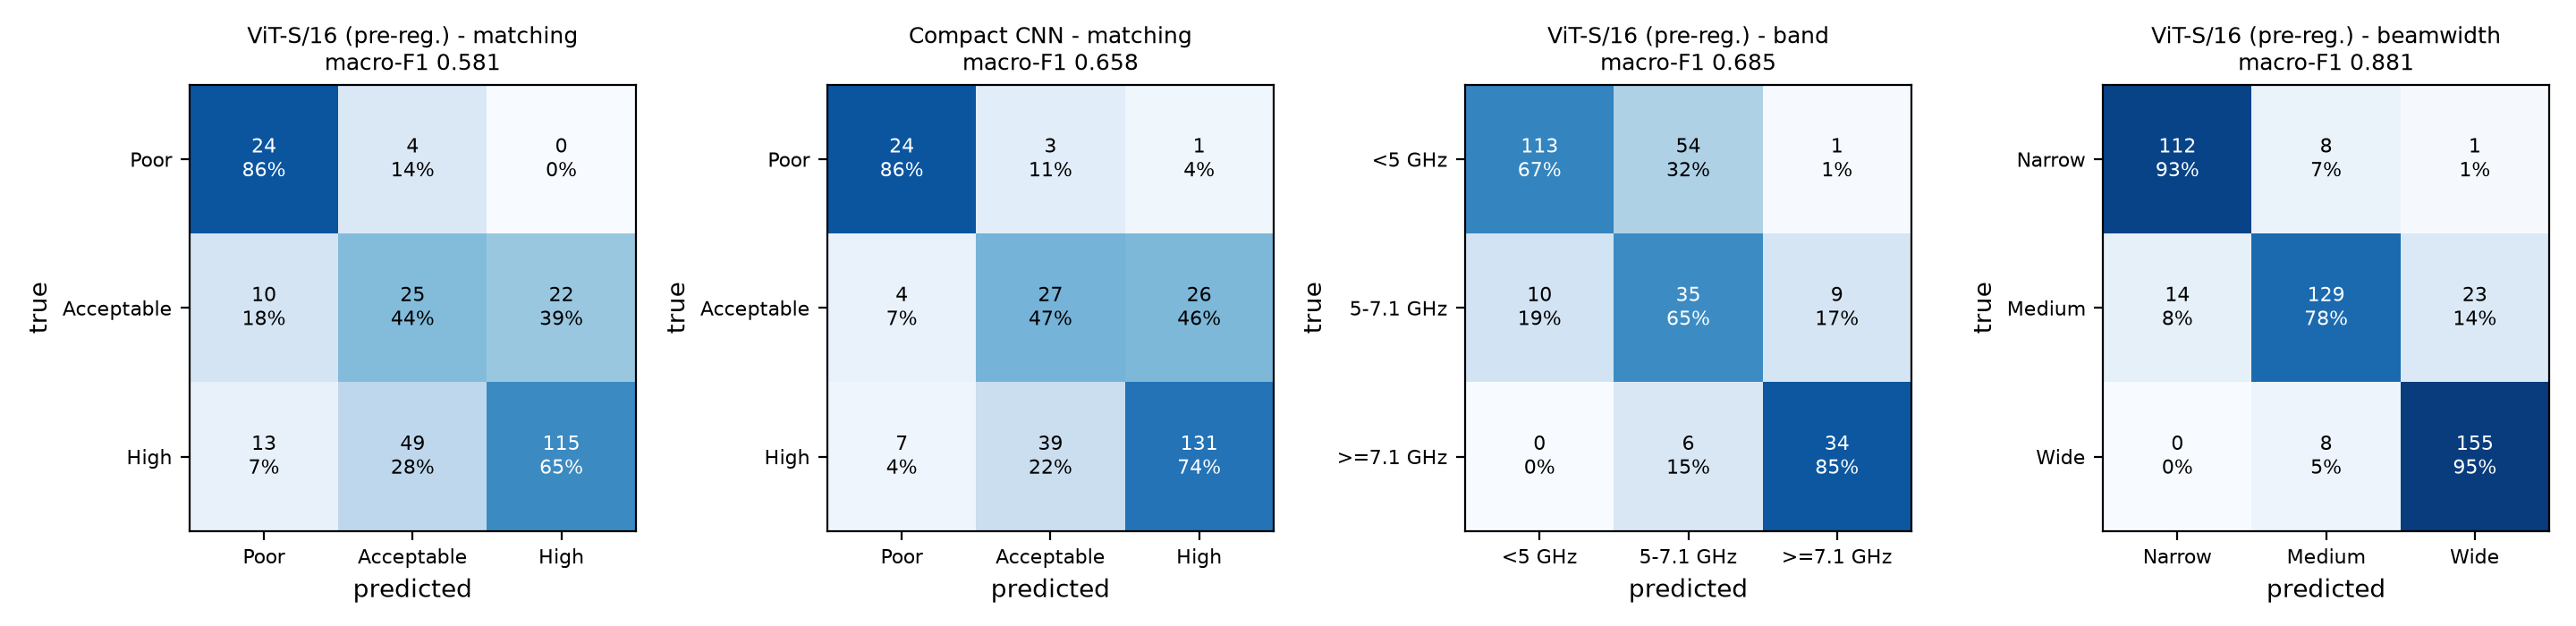
\includegraphics[width=1.00\linewidth]{../results/figures/confusion_matrices.png}
\caption*{Figure 4. Test confusion matrices (counts and row-normalised recall) for the ViT on the three tasks and the CNN on the main task.}
\end{figure}
\begin{figure}[H]\centering
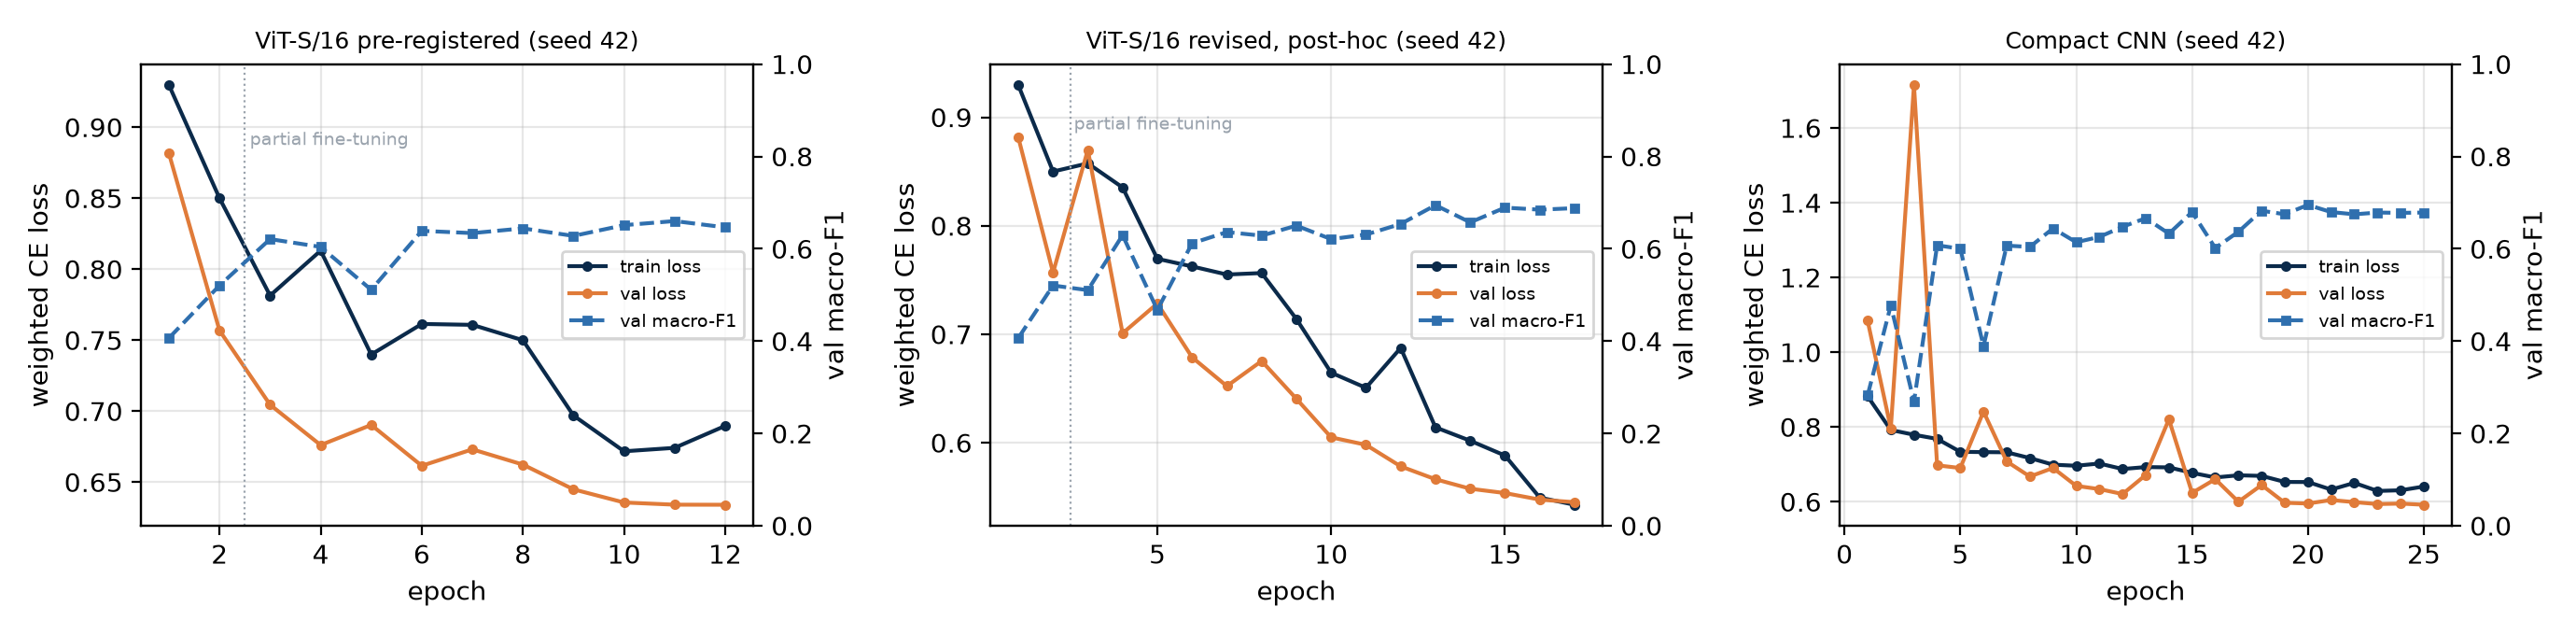
\includegraphics[width=0.95\linewidth]{../results/figures/training_curves.png}
\caption*{Figure 5. Training curves for seed 42. The dotted line marks the start of partial fine-tuning.}
\end{figure}
\subsection*{9.2 Diagnosing the underperformance: Amendment 1 and augmentation ablation}\addcontentsline{toc}{subsection}{9.2 Diagnosing the underperformance: Amendment 1 and augmentation ablation}
\begin{table}[H]\centering\small
\caption*{Table 7. Exploratory follow-up runs on the matching task (seed 42, same split; not part of the pre-registered test).}
\begin{tabularx}{\linewidth}{XXXXX}
\toprule
\textbf{Run} & \textbf{What changed} & \textbf{Val macro-F1} & \textbf{Test macro-F1} & \textbf{Test 95\% CI} \\
\midrule
ViT revised (Amendment 1) & lr 1e-4, 6 blocks, 15 epochs & 0.694 & 0.646 & [0.573, 0.707] \\
ViT, no augmentation & pre-registered optimiser, augmentation off & 0.719 & 0.725 & [0.667, 0.776] \\
CNN, no augmentation & augmentation off & 0.728 & 0.664 & [0.597, 0.723] \\
\bottomrule
\end{tabularx}
\end{table}
Under the pre-registered configuration the fine-tuned ViT scored below both the compact CNN and the frozen linear probe, so \textbf{H2 and H3 are not supported}; for seed 42 the CNN was significantly better (McNemar p = 0.0009). The training curves explain why: training accuracy plateaued near 0.70 while training loss stayed at or above validation loss, which indicates underfitting rather than overfitting. Two exploratory runs isolate the cause. (i) The revised optimisation settings of Amendment 1 raised test macro-F1 to 0.646 but failed the validation-only adoption rule (validation 0.694 against 0.702 for the probe). (ii) The augmentation ablation planned in the Module 1 report was decisive. With the pre-registered optimiser and augmentation switched off, test macro-F1 rose to \textbf{0.725} (95\% CI [0.667, 0.776]). This is statistically indistinguishable from the linear probe (McNemar p = 0.78) and numerically, but not significantly, above the CNN (p = 0.14). The CNN changed little without augmentation (0.664). The most likely mechanism is that $\pm$3$^\circ$ rotation and 2\% translation, applied with bilinear resampling, blur the one-to-two-pixel feed offset in the normalised panel, and that offset carries most of the matching information. Augmentations chosen because they are physically plausible were therefore not label-preserving at the image resolution that matters. For every model the Acceptable class was the hardest (ViT F1 0.370); it is a narrow band bounded by two thresholds on S11min, a quantity that changes sharply with feed position. The Module 2 report independently supports the underfitting diagnosis: an MLP trained on the frozen embeddings of this same ViT outperforms the ViT's own linear head.

\subsection*{9.3 Secondary task and modality comparison (RQ3)}\addcontentsline{toc}{subsection}{9.3 Secondary task and modality comparison (RQ3)}
\begin{table}[H]\centering\small
\caption*{Table 8. Test macro-F1 for the secondary image tasks (seed 42).}
\begin{tabularx}{\linewidth}{XXXXX}
\toprule
\textbf{Task / input} & \textbf{Majority} & \textbf{Compact CNN} & \textbf{ViT linear probe} & \textbf{ViT fine-tuned} \\
\midrule
Geometry $\rightarrow$ band class & 0.260 & 0.657 & 0.811 & 0.685 \\
Radiation pattern $\rightarrow$ beamwidth class & 0.180 & 0.856 & 0.884 & 0.881 \\
\bottomrule
\end{tabularx}
\end{table}
\begin{figure}[H]\centering
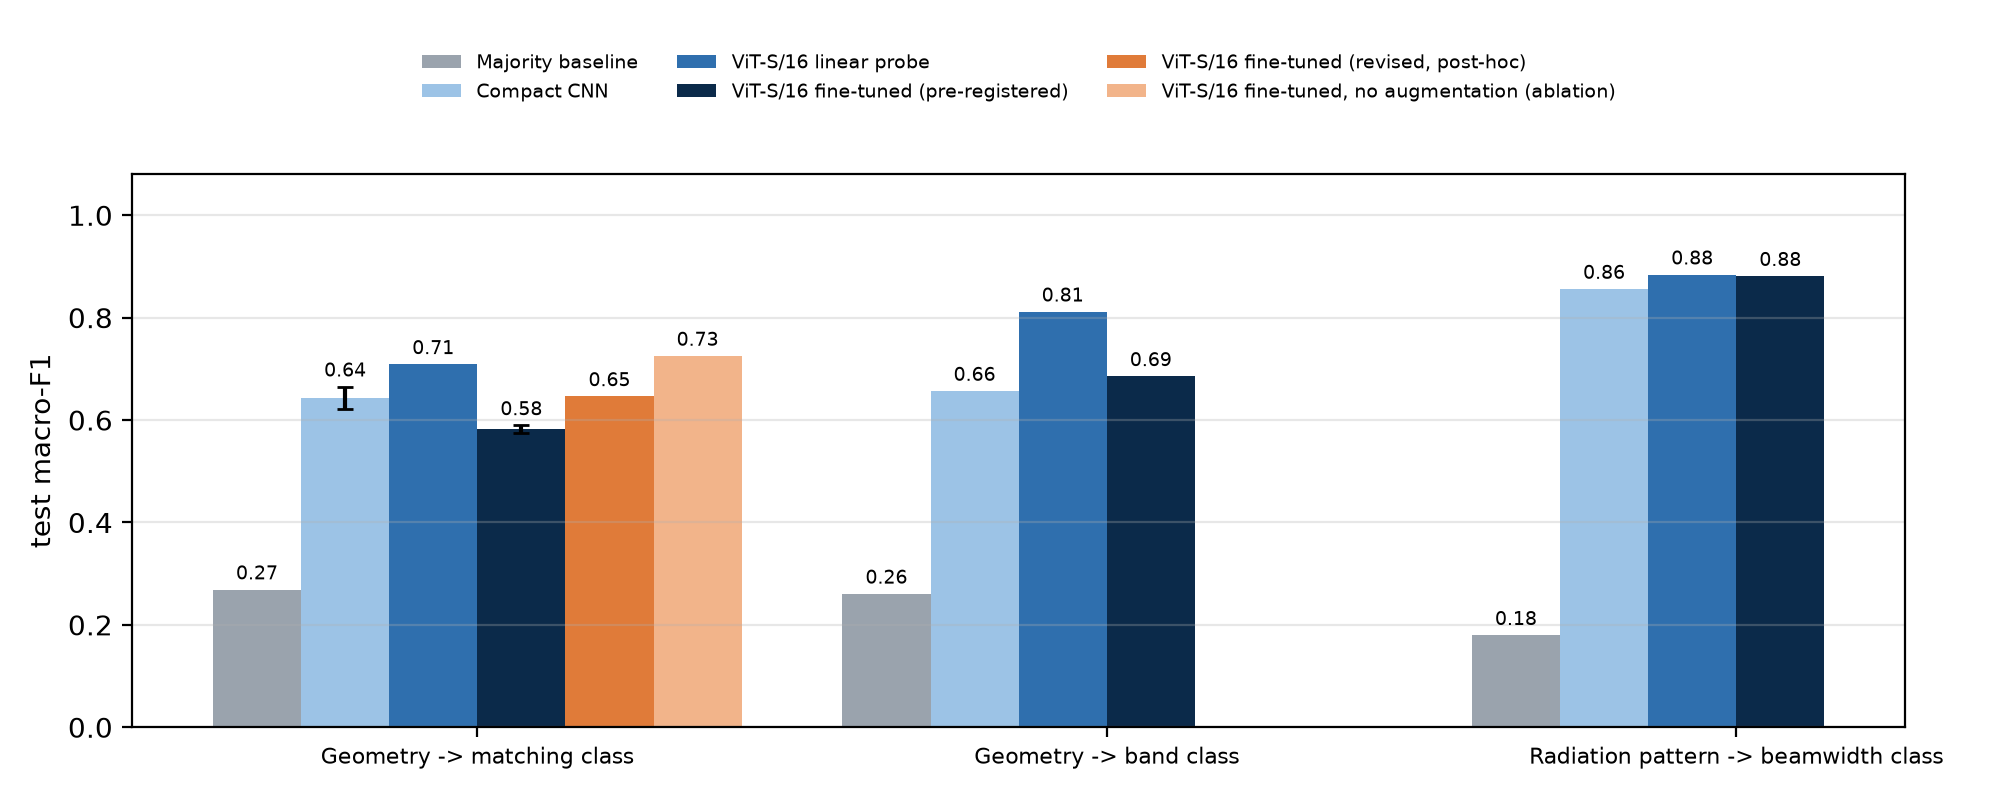
\includegraphics[width=0.95\linewidth]{../results/figures/model_comparison.png}
\caption*{Figure 6. Test macro-F1 by model and task (error bars: SD over three seeds where available).}
\end{figure}
The band class depends mainly on absolute patch size, which is visible in the top panel. The linear probe reached 0.811, ahead of the fine-tuned ViT (0.685) and the CNN (0.657). The ViT beat the majority baseline on both patch tasks, so \textbf{H1 is supported}. On radiation-pattern images all learned models performed strongly (ViT 0.881, probe 0.884, CNN 0.856), which fits beamwidth being a global shape property of the plot. These results do \textbf{not} show that radiation patterns are an intrinsically stronger modality: the RadPat task is a different, easier problem on a different dataset, so RQ3 can only be answered descriptively here. A controlled comparison needs geometry, current and field images of the same designs, which is what the proposed HFSS dataset would provide.

\subsection*{9.4 Explainability (RQ4)}\addcontentsline{toc}{subsection}{9.4 Explainability (RQ4)}
\begin{figure}[H]\centering
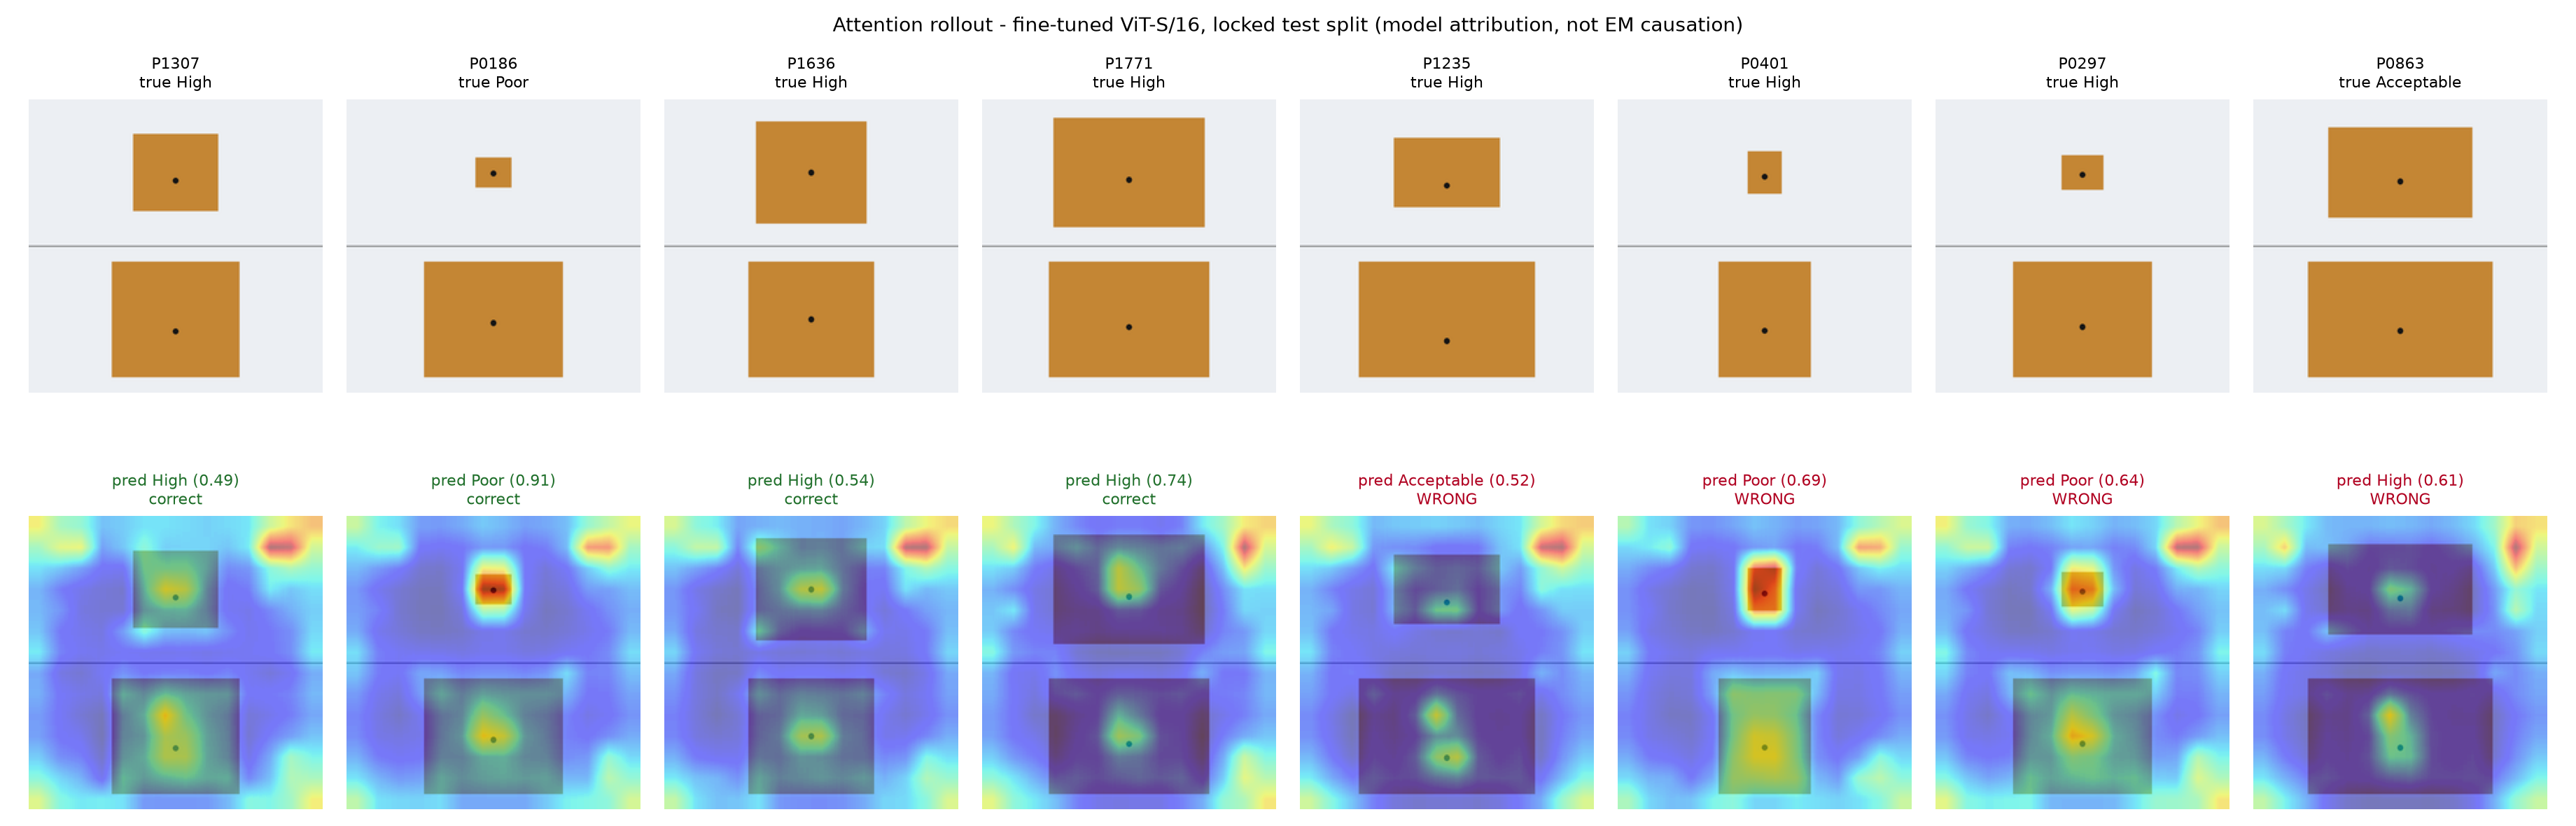
\includegraphics[width=1.00\linewidth]{../results/figures/attention_rollout_examples.png}
\caption*{Figure 7. Attention rollout on test images: four correct and four incorrect predictions (model attribution only).}
\end{figure}
\begin{figure}[H]\centering
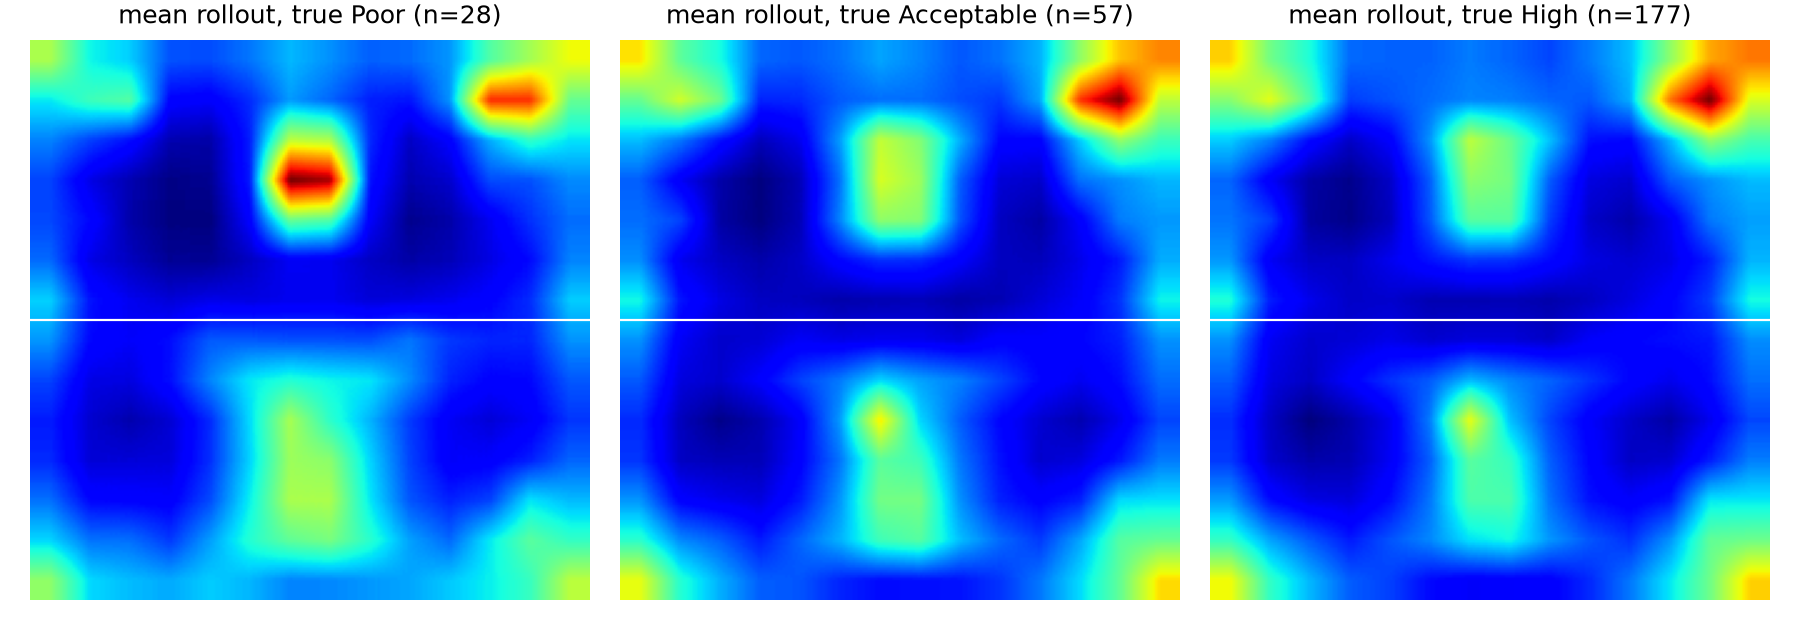
\includegraphics[width=0.87\linewidth]{../results/figures/attention_mean_by_class.png}
\caption*{Figure 8. Mean rollout map per true class over the test split.}
\end{figure}
Across the 262 test designs the patch covered on average 31.3\% of the image and received 32.0\% of the rollout mass (median enrichment 1.03). The feed halo covered 0.45\% and received 0.67\% (median enrichment 1.41); feed enrichment exceeded 1 for 100\% of designs. The top (absolute-scale) panel received 51\% of the attribution. Median feed enrichment was 1.39 for correct and 1.44 for incorrect predictions (\textbf{H4} -- Supported: patch $\times$1.03, feed halo $\times$1.41 (patch effect negligible)). The feed result is the more meaningful one: the halo covers less than 1\% of the image yet receives more attribution than its area share in every test design, which is physically plausible because feed position sets the input impedance. A patch enrichment close to 1 means attribution over the copper is roughly proportional to its area. The mean maps also show a systematic hotspot in an empty background corner of the top panel for all classes; such high-attention background tokens are a documented ViT artefact (attention sinks / register-like tokens [14]) with no electromagnetic meaning. Together these observations caution against reading attention maps as explanations of physics: they show where the model looks, not why an antenna performs as it does.

\subsection*{9.5 Robustness and out-of-distribution generalisation (RQ5)}\addcontentsline{toc}{subsection}{9.5 Robustness and out-of-distribution generalisation (RQ5)}
\begin{table}[H]\centering\small
\caption*{Table 9. Robustness of the fine-tuned ViT (seed 42) on the test split.}
\begin{tabularx}{\linewidth}{XXXX}
\toprule
\textbf{Perturbation} & \textbf{Macro-F1} & \textbf{Accuracy} & \textbf{Agreement with clean} \\
\midrule
none & 0.581 & 0.626 & 1.000 \\
translate 4px & 0.583 & 0.668 & 0.878 \\
rotate 3deg & 0.615 & 0.656 & 0.916 \\
gaussian blur r1 & 0.526 & 0.523 & 0.832 \\
contrast 0.8 & 0.581 & 0.611 & 0.962 \\
jpeg q30 & 0.575 & 0.630 & 0.939 \\
copper to grey & 0.521 & 0.565 & 0.828 \\
\bottomrule
\end{tabularx}
\end{table}
On the OOD hold-out (W/L > 1.95, n = 307, never seen in training) macro-F1 was 0.679 $\pm$ 0.027 for the ViT, 0.571 $\pm$ 0.144 for the CNN and 0.585 for the linear probe; band-class OOD macro-F1 was 0.599. \textbf{H5} -- Not supported: OOD 0.679 $\pm$ 0.027 vs test 0.582 $\pm$ 0.008 (confounded by class balance). The comparison mixes two effects. The OOD set is far more class-balanced than the test split (Poor/Acceptable/High = 80/112/115 versus 28/57/177), and macro-F1 rewards balanced recall, so the ViT's relatively good Poor and Acceptable recall counts for more on the OOD set. Covariate shift (wider patches) is therefore confounded with label shift, and the higher OOD score should not be read as better generalisation. Among the rendering perturbations, a 1-pixel Gaussian blur and recolouring the copper to grey lowered macro-F1 the most (to 0.526 and 0.521) and changed 17\% and 17\% of predictions. The model therefore relies on fine edges and on the exact colour rendering, while contrast change and JPEG compression had little effect. Applying it to real solver exports would require the fixed rendering standard set out in the Module 1 report.

\subsection*{9.6 Summary of hypotheses}\addcontentsline{toc}{subsection}{9.6 Summary of hypotheses}
\begin{table}[H]\centering\small
\caption*{Table 10. Module 1 hypothesis outcomes on the locked test split.}
\begin{tabularx}{\linewidth}{XXX}
\toprule
\textbf{ID} & \textbf{Hypothesis} & \textbf{Outcome and evidence} \\
\midrule
H1 & ViT > majority baseline (both patch tasks) & Supported: matching 0.582 vs 0.269; band 0.685 vs 0.260 \\
H2 & ViT $\geq$ compact CNN (3-seed mean, matching class) & Not supported: 0.582 $\pm$ 0.008 vs 0.643 $\pm$ 0.022; McNemar p = 0.000912 (seed 42) \\
H3 & Partial fine-tune > frozen linear probe & Not supported: 0.582 vs 0.709; McNemar p = 0.00877 \\
H4 & Attention enriched on patch and feed (median > 1) & Supported: patch $\times$1.03, feed halo $\times$1.41 (patch effect negligible) \\
H5 & Lower macro-F1 on OOD (W/L > 1.95) & Not supported: OOD 0.679 $\pm$ 0.027 vs test 0.582 $\pm$ 0.008 (confounded by class balance) \\
\bottomrule
\end{tabularx}
\end{table}
\section*{10. Ethics, Bias, Privacy, and Reproducibility}\addcontentsline{toc}{section}{10. Ethics, Bias, Privacy, and Reproducibility}
\textbf{Data rights and privacy.} Both datasets are public under licences that permit redistribution with attribution (MIT, CC BY 4.0) and contain no personal data. Attribution is given in the LICENSE file, the data card and the references. Raw archives and resized RadPat images are not redistributed; a script re-downloads them with checksums.

\textbf{Bias.} (i) Topology and material bias: a single coax-fed rectangular patch on one substrate. (ii) Frequency bias: band classes are imbalanced. (iii) Class imbalance: 67\% of training designs are High. (iv) Rendering bias: one colour scheme; probed with a colour-shift test, but the images are synthetic drawings, so real HFSS screenshot artefacts are not represented. (v) Simulation-to-reality gap: no measurements and no fabrication tolerances. (vi) Selection bias: no simulation failures were present in, or removed from, the patch data.

\textbf{Responsible use.} The classifier is a screening aid. Its confidence scores are calibrated on simulated validation data and are not guarantees of real-world performance. Any design selected with it must be verified by full-wave simulation and, for deployment, by fabrication and measurement. Attention maps are model attribution, not proof of electromagnetic causation. Training energy was kept low by using CPU-scale models, early stopping and partial fine-tuning.

\textbf{Reproducibility.} Fixed seeds; pinned dependency versions; dataset revisions, DOIs and SHA-256 checksums; locked split manifests; one configuration file; scripts for every stage; a data card and a model card; and a record of exclusions, discrepancies and deviations. The 18 automated tests cover label rules, S11 feature extraction, rendering determinism, split disjointness, the OOD rule, physical ranges and the training-only threshold derivation. All 18 pass (Appendix D).

\section*{11. Limitations and Future Work}\addcontentsline{toc}{section}{11. Limitations and Future Work}
\begin{itemize}[leftmargin=*,itemsep=1pt]
\item \textbf{Topology mismatch.} The image data are plain rectangular patches without slots or DGS, so the results do not transfer to hybrid-slotted DGS antennas.
\item \textbf{No HFSS and no field images.} Surface-current and E-field modalities could not be tested, so the geometry-versus-field comparison remains open. The geometry images are deterministic drawings, which favours the image models compared with noisy screenshots.
\item \textbf{Labels.} The -20 dB boundary is an assumption, and the classes come from simulation, not measurement.
\item \textbf{Compute.} Partial fine-tuning (4 of 12 blocks), patience 3, no hyperparameter grid, and three seeds for the main task only.
\item \textbf{Near-neighbour interpolation.} The patch sweep is dense, so test designs have close neighbours in training; the OOD hold-out partly addresses this.
\item \textbf{Modality comparison is confounded.} The radiation-pattern task uses a different dataset and label, so RQ3 is descriptive only.
\end{itemize}
\textbf{Future work.} (1) Build the HSDGS-ViT dataset described in the reference report: at least 1,000 parameterised hybrid-slotted DGS designs simulated in HFSS and automated with PyAEDT, exporting geometry, surface-current and E-field images with a fixed camera, colour map and scale and no legends. (2) Retrain the same pipeline unchanged, with augmentation limited to transforms verified to preserve the feed geometry, and add per-modality and multi-view experiments. (3) Hold out a whole slot topology and a substrate as OOD tests. (4) Obtain engineering sign-off on the -20 dB label boundary. (5) With GPU access, run full fine-tuning, the planned hyperparameter grid and five or more seeds.

\section*{12. Conclusion}\addcontentsline{toc}{section}{12. Conclusion}
Module 1 implements and executes a complete, reproducible image pipeline for the proposed framework: verified data, standardised leakage-free images, pre-registered labels and hypotheses, a pretrained ViT with three baselines, statistical comparison, quantitative explainability and robustness tests. Standardised geometry images carry a learnable signal for simulated antenna-performance classes (RQ1): every model beat the majority baseline, the best ViT variant reached a test macro-F1 of 0.725 on the matching task (no-augmentation ablation) and frozen ImageNet-21k features reached 0.811 on the band task. Under the pre-registered CPU-limited fine-tuning, however, the ViT did not outperform the compact CNN (RQ2); the decisive factor was augmentation that blurred fine feed geometry, not the architecture. Attention rollout consistently emphasised the feed region but also showed background artefacts (RQ4), and robustness tests revealed sensitivity to blur and colour rendering, with the OOD comparison confounded by label shift (RQ5). The module offers three methodological lessons for the full HFSS study: check that every augmentation preserves the label at the resolution of the relevant physical feature; always report a frozen-feature baseline; and quantify attribution against known geometry rather than inspecting heat maps. The pipeline is ready to be pointed at the HSDGS-ViT dataset, which is the step needed to test the original research claim.

\section*{Data, Code and Output Availability}\addcontentsline{toc}{section}{Data, Code and Output Availability}
All data derivatives, code, tests and outputs of Module 1 are public in the GitHub repository \url{https://github.com/rathiabeth/module1-vit-antenna-image-classification}. Each entry below links directly to the file or folder; raw third-party archives are linked at their source because they are re-downloaded with checksums rather than redistributed. Module 2 is at \url{https://github.com/rathiabeth/module2-numerical-surrogate-antenna-design}.

\begin{table}[H]\centering\small
\caption*{Table 11. Links to the data, scripts, tests and outputs of Module 1 (branch main).}
\begin{tabularx}{\linewidth}{XXX}
\toprule
\textbf{Category} & \textbf{Content} & \textbf{Link} \\
\midrule
\textbf{Data} & Patch dataset source (2,051 openEMS designs, MIT) & \href{https://huggingface.co/datasets/becklabash/rectangular-patch-antenna-freq-response}{Hugging Face, rev. 4be72a2} \\
 & RadPat-50K source (CC BY 4.0) & \href{https://doi.org/10.5281/zenodo.17067881}{Zenodo 10.5281/zenodo.17067881} \\
 & Processed design table (parameters, S11 targets, labels, split) & \href{https://github.com/rathiabeth/module1-vit-antenna-image-classification/blob/main/data/processed/patch_designs.csv}{data/processed/patch\_designs.csv} \\
 & Standardised 224 $\times$ 224 geometry images (one per design) & \href{https://github.com/rathiabeth/module1-vit-antenna-image-classification/tree/main/data/processed/patch_images}{data/processed/patch\_images} \\
 & RadPat sample table with beamwidth labels & \href{https://github.com/rathiabeth/module1-vit-antenna-image-classification/blob/main/data/processed/radpat_designs.csv}{data/processed/radpat\_designs.csv} \\
 & Locked split manifests (train / val / test / OOD) & \href{https://github.com/rathiabeth/module1-vit-antenna-image-classification/tree/main/data/splits}{data/splits} \\
 & Data dictionary and preprocessing log & \href{https://github.com/rathiabeth/module1-vit-antenna-image-classification/blob/main/data/data_dictionary.csv}{data/data\_dictionary.csv}; \href{https://github.com/rathiabeth/module1-vit-antenna-image-classification/blob/main/data/processed/preprocessing_log.json}{data/processed/preprocessing\_log.json} \\
 & Configuration (seed, thresholds, hyperparameters) & \href{https://github.com/rathiabeth/module1-vit-antenna-image-classification/blob/main/configs/default.yaml}{configs/default.yaml} \\
\textbf{Scripts} & Download and preprocessing (labels, rendering, split) & \href{https://github.com/rathiabeth/module1-vit-antenna-image-classification/blob/main/src/download_data.py}{src/download\_data.py}; \href{https://github.com/rathiabeth/module1-vit-antenna-image-classification/blob/main/src/preprocessing.py}{src/preprocessing.py}; \href{https://github.com/rathiabeth/module1-vit-antenna-image-classification/blob/main/src/dataset.py}{src/dataset.py} \\
 & ViT-S/16 fine-tuning and linear probe & \href{https://github.com/rathiabeth/module1-vit-antenna-image-classification/blob/main/src/train_vit.py}{src/train\_vit.py}; \href{https://github.com/rathiabeth/module1-vit-antenna-image-classification/blob/main/src/train_common.py}{src/train\_common.py} \\
 & Majority and compact CNN baselines & \href{https://github.com/rathiabeth/module1-vit-antenna-image-classification/blob/main/src/train_baseline.py}{src/train\_baseline.py} \\
 & Evaluation, statistics and figures & \href{https://github.com/rathiabeth/module1-vit-antenna-image-classification/blob/main/src/evaluate.py}{src/evaluate.py}; \href{https://github.com/rathiabeth/module1-vit-antenna-image-classification/blob/main/src/select_final.py}{src/select\_final.py} \\
 & Attention rollout, robustness and OOD tests & \href{https://github.com/rathiabeth/module1-vit-antenna-image-classification/blob/main/src/explainability.py}{src/explainability.py} \\
 & Full experiment queue & \href{https://github.com/rathiabeth/module1-vit-antenna-image-classification/blob/main/scripts/run_experiments.ps1}{scripts/run\_experiments.ps1}; \href{https://github.com/rathiabeth/module1-vit-antenna-image-classification/blob/main/scripts/run_experiments.sh}{scripts/run\_experiments.sh} \\
 & Report, slides, poster and diagram generators & \href{https://github.com/rathiabeth/module1-vit-antenna-image-classification/tree/main/scripts}{scripts} \\
\textbf{Tests} & Label rules, S11 extraction, rendering determinism & \href{https://github.com/rathiabeth/module1-vit-antenna-image-classification/blob/main/tests/test_preprocessing.py}{tests/test\_preprocessing.py} \\
 & Split disjointness, OOD rule, physical ranges, leakage checks & \href{https://github.com/rathiabeth/module1-vit-antenna-image-classification/blob/main/tests/test_dataset_integrity.py}{tests/test\_dataset\_integrity.py} \\
 & Stored pytest output (18 passed in 4.18s) & \href{https://github.com/rathiabeth/module1-vit-antenna-image-classification/blob/main/results/test_report.txt}{results/test\_report.txt} \\
\textbf{Outputs} & Summary table of every model and split & \href{https://github.com/rathiabeth/module1-vit-antenna-image-classification/blob/main/results/metrics/summary_table.csv}{results/metrics/summary\_table.csv} \\
 & Per-run metrics, training histories, McNemar and bootstrap tests & \href{https://github.com/rathiabeth/module1-vit-antenna-image-classification/tree/main/results/metrics}{results/metrics} \\
 & Per-design test predictions with calibrated confidence & \href{https://github.com/rathiabeth/module1-vit-antenna-image-classification/tree/main/results/predictions}{results/predictions} \\
 & Explainability summary (attention enrichment, robustness) & \href{https://github.com/rathiabeth/module1-vit-antenna-image-classification/blob/main/results/metrics/explainability_summary.json}{results/metrics/explainability\_summary.json} \\
 & All figures used in this report & \href{https://github.com/rathiabeth/module1-vit-antenna-image-classification/tree/main/results/figures}{results/figures} \\
 & Image embeddings handed to Module 2 & \href{https://github.com/rathiabeth/module1-vit-antenna-image-classification/tree/main/results/features}{results/features} \\
 & Report, slides and poster & \href{https://github.com/rathiabeth/module1-vit-antenna-image-classification/tree/main/reports}{reports}; \href{https://github.com/rathiabeth/module1-vit-antenna-image-classification/tree/main/presentations}{presentations}; \href{https://github.com/rathiabeth/module1-vit-antenna-image-classification/tree/main/poster}{poster} \\
\bottomrule
\end{tabularx}
\end{table}
\section*{References}\addcontentsline{toc}{section}{References}
\begin{enumerate}[leftmargin=*,itemsep=1pt]
\item A. Dosovitskiy et al., "An image is worth 16x16 words: Transformers for image recognition at scale," in Proc. ICLR, 2021, arXiv:2010.11929.
\item B. LaBash et al., "Improving generative inverse design of rectangular patch antennas with test time optimization," arXiv:2505.18188, 2025. Dataset: huggingface.co/datasets/becklabash/rectangular-patch-antenna-freq-response (MIT), rev. 4be72a2.
\item C. M. Bhuma, P. Sure, S. K. Painam, J. Chandrasekhar Rao and U. Srinivasa Rao, "RadPat-50K: A large-scale benchmark for antenna array radiation patterns," Zenodo, v1.1, 2025, doi:10.5281/zenodo.17067881 (CC BY 4.0).
\item C. A. Balanis, Antenna Theory: Analysis and Design, 4th ed. Hoboken, NJ: Wiley, 2016.
\item 3GPP, "NR; User Equipment (UE) radio transmission and reception; Part 1: Range 1 Standalone," TS 38.101-1.
\item R. Wightman, "PyTorch Image Models (timm)," GitHub repository, 2019--2026; A. Steiner et al., "How to train your ViT? Data, augmentation, and regularization in vision transformers," TMLR, 2022.
\item S. Abnar and W. Zuidema, "Quantifying attention flow in transformers," in Proc. ACL, 2020, pp. 4190--4197.
\item C. Guo, G. Pleiss, Y. Sun and K. Q. Weinberger, "On calibration of modern neural networks," in Proc. ICML, 2017.
\item A. Paszke et al., "PyTorch: An imperative style, high-performance deep learning library," in Proc. NeurIPS, 2019.
\item H. Touvron et al., "Training data-efficient image transformers \& distillation through attention," in Proc. ICML, 2021.
\item T. Liebig et al., openEMS -- a free and open electromagnetic field solver, \url{https://openems.de}.
\item Q. McNemar, "Note on the sampling error of the difference between correlated proportions or percentages," Psychometrika, vol. 12, pp. 153--157, 1947.
\item B. Efron and R. J. Tibshirani, An Introduction to the Bootstrap. New York: Chapman \& Hall, 1993.
\item T. Darcet, M. Oquab, J. Mairal and P. Bojanowski, "Vision transformers need registers," in Proc. ICLR, 2024.
\end{enumerate}
\newpage
\section*{Appendix A. Data Dictionary}\addcontentsline{toc}{section}{Appendix A. Data Dictionary}
\begin{table}[H]\centering\small
\caption*{Table 12. Data dictionary (data/data\_dictionary.csv).}
\begin{tabularx}{\linewidth}{XXXXX}
\toprule
\textbf{Dataset} & \textbf{Variable} & \textbf{Type} & \textbf{Unit} & \textbf{Description} \\
\midrule
patch & design\_id & string & - & Unique design key (P + source id); one image per design \\
patch & length\_mm & float & mm & Patch length L (resonant dimension) \\
patch & width\_mm & float & mm & Patch width W \\
patch & feed\_y\_mm & float & mm & Coaxial feed offset from patch centre along L (negative toward edge) \\
patch & f\_res\_ghz & float & GHz & First matched resonance: lowest-frequency local S11 minimum below -10 dB (global minimum if never matched) \\
patch & f\_deepest\_ghz & float & GHz & Frequency of the deepest S11 dip in 1-10 GHz (often a higher-order mode) \\
patch & s11\_min\_db & float & dB & Global minimum simulated S11 over 1-10 GHz (openEMS FDTD); defines perf\_class \\
patch & s11\_at\_res\_db & float & dB & Simulated S11 at f\_res \\
patch & bw10\_mhz & float & MHz & Contiguous -10 dB bandwidth around resonance (0 if unmatched) \\
patch & fbw10\_pct & float & \% & Fractional -10 dB bandwidth \\
patch & wl\_ratio & float & - & W/L aspect ratio \\
patch & feed\_ratio & float & - & Feed offset normalised by L/2 (0 centre, 1 edge) \\
patch & area\_mm2 & float & mm\textasciicircum{}2 & Patch area W x L \\
patch & perf\_class & int & 0/1/2 & Poor (S11min > -10 dB), Acceptable (-20 < S11min <= -10), High (S11min <= -20 dB) \\
patch & band\_class & int & 0/1/2 & f\_res < 5 GHz | 5-7.125 GHz | >= 7.125 GHz (3GPP FR1 / FR3 boundary) \\
patch & split & category & train/val/test/ood & Locked design-level allocation (seed 42) \\
patch & image\_path & string & - & Rendered standardised geometry image (224x224 PNG) \\
radpat & design\_id & string & - & R + RadPat sample id \\
radpat & N & int & - & Number of array elements \\
radpat & spacing\_wavelengths & float & lambda & Element spacing \\
radpat & weights & category & - & Amplitude taper (uniform, binomial, cosine, kaiser, hamming, hann, blackman, exponential) \\
radpat & steering\_deg\_nominal & float & deg & Nominal steering angle \\
radpat & HPBW\_deg & float & deg & Half-power beamwidth reported by dataset authors \\
radpat & D\_peak\_dBi & float & dBi & Peak directivity; value -120 is a sentinel (not used as label) \\
radpat & hpbw\_class & int & 0/1/2 & Narrow/Medium/Wide beam from training-split HPBW terciles \\
\bottomrule
\end{tabularx}
\end{table}
\section*{Appendix B. Configuration}\addcontentsline{toc}{section}{Appendix B. Configuration}
\begin{verbatim}
# Module 1 - Vision Transformer image module. Central configuration: every script in src/ reads this file.
seed: 42
num_threads: 4

paths:
  raw: data/raw
  processed: data/processed
  splits: data/splits
  results: results
  checkpoints: results/checkpoints   # git-ignored

datasets:
  patch:
    # Hugging Face: becklabash/rectangular-patch-antenna-freq-response (MIT licence)
    repo_id: becklabash/rectangular-patch-antenna-freq-response
    revision: 4be72a22e55fbf46966c59a5d6b3ec95c836379b
    file: data/train-00000-of-00001.parquet
  radpat:
    # Zenodo record 17067881 (RadPat-50K v1.1, CC-BY-4.0); only the 10K polar subset is used
    record: 17067881
    metadata_file: Metadata_10K.csv
    images_zip: Polar_10K.zip
    subsample: 3000

labels:
  # Matching thresholds. -10 dB (VSWR ~1.92) is the conventional impedance-bandwidth criterion.
  # -20 dB as the "high" boundary is a project ASSUMPTION that requires engineering confirmation.
  s11_matched_db: -10.0
  s11_high_db: -20.0
  # Band edges (GHz) from 3GPP TS 38.101-1 (FR1 upper edge 7.125 GHz; n77 3.3-4.2, n79 4.4-5.0).
  band_edges_ghz: [5.0, 7.125]
  band_names: ["FR1_mid_below5GHz", "FR1_upper_5to7GHz", "FR3_6Gcandidate_above7GHz"]
  perf_names: ["Poor", "Acceptable", "High"]
  hpbw_names: ["Narrow", "Medium", "Wide"]

split:
  train: 0.70
  val: 0.15
  test: 0.15
  # Out-of-distribution hold-out: the widest patches (W/L ratio above this) never enter train/val/test.
  ood_wl_ratio_min: 1.95

render:
  size: 224          # final image size (pixels)
  supersample: 4     # render at 4x then downsample (anti-aliasing keeps sub-pixel feed position)

vit:
  model_name: vit_small_patch16_224.augreg_in21k_ft_in1k
  batch_size: 16
  warmup_epochs: 2         # stage A: head only
  finetune_epochs: 10      # stage B: head + last N blocks
  unfreeze_blocks: 4
  lr_head: 1.0e-3
  lr_backbone: 3.0e-5
  weight_decay: 0.01
  dropout: 0.1
  patience: 3              # early stopping on validation macro-F1 (reduced from 8 for CPU budget)

# POST-HOC REVISION (added 25 Oct 2026 after the pre-registered seed-42 run). That run underfitted:
# train acc ~0.70, still rising; best val macro-F1 0.660 < linear-probe val 0.702. Its test score had been
# printed before this decision, which is disclosed in docs/HYPOTHESES.md. Only optimisation settings change
# (labels, split, augmentation and data are unchanged). The revision is adopted only if its VALIDATION macro-F1
# beats both the pre-registered config and the linear probe.
vit_revised:
  model_name: vit_small_patch16_224.augreg_in21k_ft_in1k
  batch_size: 16
  warmup_epochs: 2
  finetune_epochs: 15
  unfreeze_blocks: 6
  lr_head: 1.0e-3
  lr_backbone: 1.0e-4
  weight_decay: 0.01
  dropout: 0.1
  patience: 5

cnn:
  batch_size: 32
  epochs: 25
  lr: 1.0e-3
  weight_decay: 1.0e-4
  patience: 5

\end{verbatim}
\section*{Appendix C. Experimental Details}\addcontentsline{toc}{section}{Appendix C. Experimental Details}
\begin{table}[H]\centering\small
\caption*{Table 13. Every executed classification run (test split).}
\begin{tabularx}{\linewidth}{XXXXXXXX}
\toprule
\textbf{Dataset} & \textbf{Task} & \textbf{Mode} & \textbf{Seed} & \textbf{Macro-F1} & \textbf{Accuracy} & \textbf{ECE} & \textbf{Train time (min)} \\
\midrule
patch & band\_class & majority & -- & 0.260 & 0.641 & 0.012 & -- \\
patch & band\_class & cnn & 42 & 0.657 & 0.737 & 0.062 & 2.5 \\
patch & band\_class & linear\_probe & -- & 0.811 & 0.851 & 0.049 & -- \\
patch & band\_class & finetune & 42 & 0.685 & 0.695 & 0.039 & 14.6 \\
patch & perf\_class & majority & -- & 0.269 & 0.676 & 0.000 & -- \\
patch & perf\_class & cnn & 42 & 0.658 & 0.695 & 0.061 & 9.7 \\
patch & perf\_class & cnn & 43 & 0.654 & 0.691 & 0.084 & 19.3 \\
patch & perf\_class & cnn & 44 & 0.618 & 0.641 & 0.044 & 2.8 \\
patch & perf\_class & cnn\_noaug & 42 & 0.664 & 0.740 & 0.048 & 9.6 \\
patch & perf\_class & linear\_probe & -- & 0.709 & 0.718 & 0.057 & -- \\
patch & perf\_class & finetune & 42 & 0.581 & 0.626 & 0.066 & 25.4 \\
patch & perf\_class & finetune & 43 & 0.575 & 0.607 & 0.062 & 37.9 \\
patch & perf\_class & finetune & 44 & 0.590 & 0.634 & 0.058 & 49.2 \\
patch & perf\_class & finetune\_revised & 42 & 0.646 & 0.683 & 0.062 & 77.4 \\
patch & perf\_class & finetune\_noaug & 42 & 0.725 & 0.729 & 0.084 & 25.1 \\
radpat & hpbw\_class & majority & -- & 0.180 & 0.369 & 0.032 & -- \\
radpat & hpbw\_class & cnn & 42 & 0.856 & 0.856 & 0.099 & 6.1 \\
radpat & hpbw\_class & linear\_probe & -- & 0.884 & 0.882 & 0.013 & -- \\
radpat & hpbw\_class & finetune & 42 & 0.881 & 0.880 & 0.024 & 28.2 \\
\bottomrule
\end{tabularx}
\end{table}
Failed or abandoned runs: the first CNN design (four double-convolution blocks at full resolution, about 60 s per epoch) was stopped after three epochs to save compute and replaced by the stride-2 stem version reported here. A first training queue was restarted as a detached, resumable process; partial runs were discarded and re-run from scratch. Because of a launcher quoting error, the pre-registered ViT seeds 43 and 44 and CNN seed 43 ran concurrently with other jobs; their results are unaffected, but their training times are inflated and should not be compared. The first definition of resonance (the deepest S11 dip) was replaced before training by the first matched resonance. No test-set result was used for any of these decisions.

\section*{Appendix D. Reproducibility Instructions}\addcontentsline{toc}{section}{Appendix D. Reproducibility Instructions}
\begin{verbatim}
python -m venv .venv && .venv\Scripts\activate
pip install -r requirements.txt --extra-index-url https://download.pytorch.org/whl/cpu
python -m src.download_data          # ~510 MB (add --skip-radpat for ~10 MB)
python -m src.preprocessing
pytest -q
powershell -File scripts\run_experiments.ps1      # or: bash scripts/run_experiments.sh  (~4 h on CPU)
python scripts/make_deliverables.py
\end{verbatim}
Repository: \url{https://github.com/rathiabeth/module1-vit-antenna-image-classification}. The pytest output (18 passed in 4.18s) is stored in \href{https://github.com/rathiabeth/module1-vit-antenna-image-classification/blob/main/results/test_report.txt}{results/test\_report.txt}; environment, runtimes and determinism notes are in \href{https://github.com/rathiabeth/module1-vit-antenna-image-classification/blob/main/docs/REPRODUCIBILITY.md}{docs/REPRODUCIBILITY.md}. All links are listed in the section Data, Code and Output Availability.

\end{document}